\clearpage
\noindent\makebox[0pt][l]{\fontsize{13}{16}\selectfont 478}\hfill{\small\textbf{NACHLASS.}}\hfill\null\par
\vspace*{32mm}
\begin{center}
{\Large\bfseries NACHLASS.}\par\vspace{15mm}
[1.]\par\medskip
\textbf{Einfluss unvollkommner Berichtigung am ersten Heliotrop.}
\end{center}
Grösserer Einfachheit wegen nehmen wir an, dass die Richtung der Axe
horizontal und zum Azimuth 0 gerichtet ist, der leuchtende Punkt aber gleichfalls
im Horizont im Azimuth $A$ liegt. Die Fehler sind nun doppelter Art:

\noindent I. Rücksichtlich des Azimuths.
\begin{list}{}{\setlength{\leftmargin}{9mm}\setlength{\labelwidth}{6mm}\setlength{\itemsep}{2pt}\setlength{\parsep}{0pt}\setlength{\topsep}{3pt}}
\item[1.] Wenn das Fadennetz um $\alpha$ zu weit rechts steht,
wird das Licht nicht in das Azimuth 0, sondern
in das Azimuth $-\alpha$ reflectirt. Also die Wirkung $=-\alpha$
\item[2.] Ist der Spiegel von der senkrechten Lage gegen
die Führungsstange um $\beta$ vorwärts gedreht, so
entsteht daraus die Wirkung\hfill $=+2\beta$
\item[3.] Ist die Axe der Hülse zu weit von der Fernrohraxe
entfernt, im Verhältniss $(1+\gamma):1$, so ist die
Wirkung\hfill $=+206265.\gamma.\operatorname{tg}\frac12 A$
\end{list}
\noindent II. Rücksichtlich der Höhe.
\begin{list}{}{\setlength{\leftmargin}{9mm}\setlength{\labelwidth}{6mm}\setlength{\itemsep}{2pt}\setlength{\parsep}{0pt}\setlength{\topsep}{3pt}}
\item[4.] Ist der Spiegel nach oben zu gerichtet um $\delta$
(die Schraube zu stark angezogen):\hfill $+2\delta\cos\frac12 A$
\item[5.] Die Spiegelaxe unten zu weit vorwärts gelehnt
um $\varepsilon$:\hfill $+2\varepsilon\cos\frac12 A^2$
\item[6.] Die Spiegelaxe unten zu weit rechts um $\zeta$:\hfill $+\zeta\sin A$
\end{list}

\clearpage
\noindent\null\hfill{\small\textbf{HELIOTROP.}}\hfill\makebox[0pt][r]{\fontsize{13}{16}\selectfont 479}\par\medskip
\begin{list}{}{\setlength{\leftmargin}{9mm}\setlength{\labelwidth}{6mm}\setlength{\itemsep}{2pt}\setlength{\parsep}{0pt}\setlength{\topsep}{0pt}}
\item[7.] Die Fernrohraxe unten zu weit vorwärts um $\eta$,
so dass doch die optische Axe der Hauptaxe
parallel werden kann:\hfill $+2\eta\sin\frac12 A^2$
\item[8.] Das Fadennetz zu hoch um $\theta$:\hfill $+\theta$
\end{list}
\noindent Noch ist für das Azimuth nachzuholen\par
\hspace*{9mm}Wirkung der Parallaxe $\pi$:\hfill $-\pi\sin A.$
\begin{center}\textbf{Für den zweiten Heliotrop.}\end{center}
Für das Azimuth kommt bloss die Neigung der beiden Spiegel gegen
einander in Frage. Ist der kleine Spiegel zu weit vorwärts gedreht um $\alpha$, so
wird das Bild nach $-2\alpha$ hin reflectirt.
\begin{center}
[2.]\par\medskip
\textbf{Zur Berichtigung des Heliotrops.}
\end{center}
1. Ein wesentliches Bedürfniss für die Berichtigung des Heliotrops sind
ein paar Stative, wovon wenigstens das eine in der Höhe stellbar ist, und
denen man mit Leichtigkeit und Genauigkeit jede erforderliche Höhenungleichheit
verschaffen kann.\ .\ .\ .\ .\ .\ .

2. Die einfachste Bestimmung des geometrischen Orts des Spiegelbildes
eines ruhenden Gegenstandes, während der an einer Axe festsitzende Spiegel
sich um diese dreht, ist folgende:

Es sei $A$ der Schnitt der Spiegel\textls[120]{fläche} mit der Drehungsaxe, $B$ ein
Punkt in der Normalen gegen die Spiegelfläche, und zwar auf der Rückseite
des Spiegels, $AB$ willkürlich. Es ist also $B$ fest gegen den Spiegel, beschreibt
aber bei dessen Drehung im Raume einen Kreis, und zwar in demselben
Sinn wie irgend ein anderer zum Spiegel fester Punkt, z.\,B. die Mitte
einer der vier Seiten seiner rectangularen Begrenzung. Zugleich ist der Mittelpunkt
jenes Kreises $C$ in der Drehungsaxe, und $AC=AB\cos\theta$, wenn $90^\circ-\theta$
die Neigung des Spiegels gegen die Drehungsaxe bedeutet. Nun wird das
Spiegelbild $P$ von einem im Raume festen Punkt $D$ gefunden, wenn man
durch $D$ eine Parallele mit $AB$ zieht, und nöthigenfalls sie so weit verlängert,
bis $AP=AD$. Das bisher willkürliche $AB$ kann man so gross annehmen,
dass $AC=AE$ wird, wenn $DE$ auf die Drehungsaxe $AE$ normal gezogen ist.

\clearpage
\noindent\makebox[0pt][l]{\fontsize{13}{16}\selectfont 480}\hfill{\small\textbf{NACHLASS.}}\hfill\null\par
\begin{center}
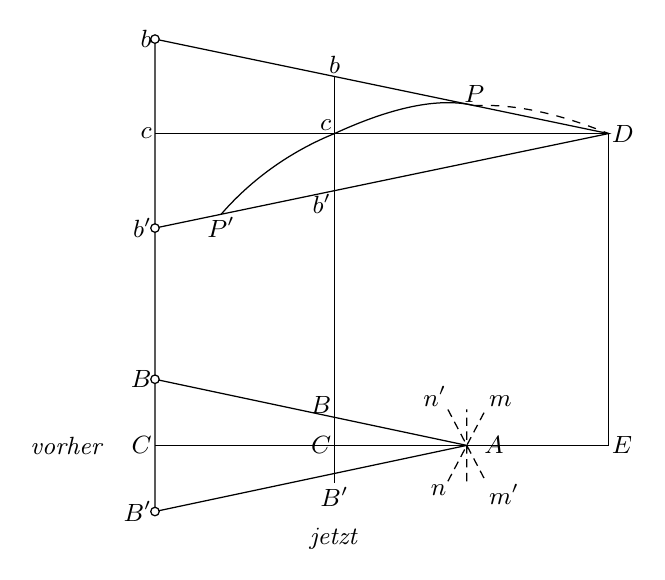
\begin{tikzpicture}[x=12mm,y=12mm,line width=.45pt,every node/.style={font=\small,inner sep=1pt}]
\draw (0,0)--(0,5)--(4.8,4)--(0,3)--cycle;
\draw (0,4)--(4.8,4)--(4.8,.7)--(0,.7);
\draw (0,1.4)--(3.3,.7)--(0,0);
\draw (1.9,4.604)--(1.9,.297);
\draw (.7,3.146) .. controls (1.05,3.55) and (1.48,3.83) .. (1.9,4) .. controls (2.40,4.23) and (2.95,4.40) .. (3.38,4.296);
\draw[dashed] (3.38,4.296) .. controls (3.9,4.32) and (4.4,4.16) .. (4.8,4);
\draw[densely dashed] (3.10,.32)--(3.50,1.08) (3.10,1.08)--(3.50,.32) (3.3,.32)--(3.3,1.08);
\foreach \q in {(0,5),(0,3),(0,1.4),(0,0)} \draw[fill=white] \q circle (.045);
\node[left] at (0,5) {$b$}; \node[left] at (0,4) {$c$};
\node[left] at (0,3) {$b'$}; \node[left] at (0,1.4) {$B$};
\node[left] at (0,.7) {$C$}; \node[left] at (0,0) {$B'$};
\node[above] at (1.9,4.604) {$b$}; \node[above left] at (1.9,4) {$c$};
\node[below left] at (1.9,3.396) {$b'$};
\node[above left] at (1.9,.997) {$B$}; \node[left] at (1.9,.7) {$C$};
\node[below] at (1.9,.297) {$B'$};
\node[above] at (3.38,4.296) {$P$}; \node[below] at (.7,3.146) {$P'$};
\node[right] at (4.8,4) {$D$}; \node[right] at (4.8,.7) {$E$};
\node[right] at (3.45,.7) {$A$};
\node[above left] at (3.12,1.08) {$n'$}; \node[above right] at (3.5,1.08) {$m$};
\node[below left] at (3.12,.32) {$n$}; \node[below right] at (3.5,.32) {$m'$};
\node[left] at (-.5,.7) {\textit{vorher}};
\node[below] at (1.9,-.14) {\textit{jetzt}};
\end{tikzpicture}
\end{center}
Zieht man dann $Dc$ mit $AC$ und $Cc$ mit $ED$ parallel, so ist $Dc=2AC$,
$Ac=AD$, also $c$ auf der Oberfläche einer mit Radius $AD$ um $A$ beschriebenen
Kugel. Legt man durch $c$ eine gegen $Dc$ normale Ebene, und beschreibt
darin mit Halbmesser $cb=2CB$ um $c$ einen Kreis $bb'$, so liegt
$PP'$ in der Oberfläche des geraden Kegels, dessen Spitze $D$, Axe $Dc$, Seiten
$Db$, $Db'$, Öffnungswinkel $bDb'=BAB'=2\theta$. Auf der Kugelfläche selbst ist
der Weg von $P$ zwar keine sphärische Ellipse\begingroup\renewcommand{\thefootnote}{*)}\footnote{Unter sphärischer Ellipse verstehe ich diejenige Curve auf der Kugelfläche, von welcher jede centrale Projection eine Ellipse ist; die hier in Rede stehende hingegen ist eine solche, von welcher eine stereographische Projection eine Ellipse ist.}\endgroup,\ .
aber doch sehr wenig davon verschieden. Der Durchmesser, in dessen Fortsetzung $D$ liegt, ist genau $=4\theta$;
der dagegen senkrechte sehr nahe $2\theta.\frac{cD}{Ac}=4\theta.\frac{AE}{AD}$.
Dieses Bild dreht sich um seinen Mittelpunkt in demselben Sinn, wie $b$ um den seinigen $c$ für
einen Betrachter innerhalb des Raumes $DcC$, oder wie ein Punkt $m$ oder $n$
für einen Betrachter vor dem Spiegel, und diese Gleichheit des Sinnes der
Drehung gilt, man mag das Bild mit blossem Auge oder durch ein umkehrendes
Fernrohr sehen.

3. Es ist nun leicht, diese Sätze zu benutzen, um den kleinen Spiegel
gegen die Drehungsaxe normal zu bringen, möge dies nun für die vom Fernrohr
abgekehrte oder für die ihm zugekehrte Lage verlangt werden.

Eine ganz rohe Annäherung, z.\,B. auf 5--10 Grad, bewirkt man ohne
weiteres nach dem Augenmaass. Man stelle dann das Fernrohr so, dass die

\clearpage
\noindent\null\hfill{\small\textbf{HELIOTROP.}}\hfill\makebox[0pt][r]{\fontsize{13}{16}\selectfont 481}\par\medskip
\noindent Spiegelaxe nach dem Augenmaass vertical steht und betrachte mit blossem
Auge das Bild eines schicklichen Gegenstandes. Wenn nun bei einer Drehung
des Fernrohrs das Bild nicht ruhig bleibt, so muss man diejenige verticale
Seitenwand des Spiegels von sich \textls[120]{abdrehen}, welche mit dem Bilde gleichnamige
Bewegung zeigt, d.\,i. die steigende Seite, wenn das Bild steigt, die
sinkende, wenn es sinkt. Dies wiederholt man jedesmal, von der nahe verticalen
Lage der Spiegelwand anfangend, bis das blosse Auge keine Bewegung
des Bildes mehr erkennt.

Man wiederholt nun dieses Geschäft, indem man dem Spiegel gegenüber
ein Fernrohr aufstellt. Ist der Fehler noch so gross, dass das Bild bei der
Drehung das Gesichtsfeld verlassen würde, so muss zugleich das Fernrohr gedreht
und nöthigenfalls mit seinem Stativ verschoben werden. Um im voraus
zu beurtheilen, wie viel etwa und in welchem Sinn das Hülfsfernrohr gedreht
und verschoben werden muss, ist vor allem nöthig, den Sinn der beiden möglichen
Drehungen ein für allemal zweckmässig zu unterscheiden.

Ich nenne eine positive Drehung die, in der die Gewinde einer auf gewöhnliche
Art geschnittenen Schraube sich von dem in der Axe der Schraube
gedachten Betrachter entfernen. Durch eine solche Drehung schraubt man
also eine Schraube in die Mutter, oder zieht die Mutter an. Bei einer Drehung
um eine verticale Axe, den Betrachter oberhalb des gedrehten angenommen,
geht also die positive Bewegung in dem Sinne der täglichen Sonnenbewegung
für die nördliche Hemisphäre; bei Drehung um eine horizontale Axe
geht die Bewegung in der Ordnung Links, Oben, Rechts, Unten: L.O.R.U,
O.R.U.L, R.U.L.O, U.L.O.R; negative wäre L.U.R.O, U.R.O.L, R.O.L.U,
O.L.U.R.

Die allgemeine Regel ist nun folgende.

Es sei $e$ die Neigung der nach dem Gegenstande gehenden Geraden gegen
die Spiegelebene, $p$ eine kleine Drehung des Fernrohrs um seine Axe (wobei
der positive Sinn nach der Stellung des Betrachters vor dem Spiegel, also an
der Ocularseite des Heliotropfernrohrs, dann wenn der Spiegel dem Fernrohr
zugekehrt bleiben soll, und vice versa im umgekehrten Fall, zu beurtheilen
ist), und \textls[120]{steigt} das Bild bei dieser Drehung um $h$ für das blosse Auge, oder
sinkt so viel beim Sehen durch das Hülfsfernrohr, so muss behuf der Berichtigung
gedreht werden um die Grösse
\vfill\noindent IX.\hfill61

\clearpage
\noindent\makebox[0pt][l]{\fontsize{13}{16}\selectfont 482}\hfill{\small\textbf{NACHLASS.\quad HELIOTROP.}}\hfill\null\par
\[
\frac{h}{\sin e\sin p}
\]
\[
\left.\begin{aligned}
&\text{1) der Spiegel um die Spiegelaxe}\\
&\text{2) das Hülfsfernrohr ebenso viel um diese}
\end{aligned}\right\}\ \text{von oben her betrachtet.}
\]
Die letztere Bewegung geschieht durch Drehung der Alhidade des Fernrohrs
um die Verticalaxe des Theodolithen (wenn das Hülfsfernrohr an einem
solchen sitzt) und ausserdem durch Verschiebung um
\[
\frac{h}{4\sin e\sin p}\times\delta,
\]
wenn $\delta$ die Entfernung der Spiegelaxe von der Theodolithenaxe bedeutet.

$h$ ist übrigens leicht zu schätzen, wenn der Halbmesser des Gesichtsfeldes
bekannt ist; bei dem kleinen Theodolithen ist der Durchmesser $=58'$.
In der Ausübung wird aber eine Rechnung nie nöthig, sondern zureichend sein,
nur den Sinn der erforderlichen Drehungen voraus zu bestimmen.

4. Von den übrigen bei Berichtigung des Heliotrops vorkommenden
Operationen braucht hier nur noch eine erwähnt zu werden, nemlich die, wodurch
Heliotropfernrohr und Hülfsfernrohr in entgegengesetzt parallele Lage
gebracht werden, mit einem Abstande der Parallelen, welcher der halben Distanz
der Mittelpunkte der grossen Spiegel gleich sein soll. Früher geschah
dies so, dass man zuerst das Heliotropfernrohr auf einen Gegenstand richtete
und verkehrt wieder in die Pfannen legte, vor der Wiedereinlegung aber das
Hülfsfernrohr in angemessener Höhe auf dasselbe Object richtete.

Jetzt ändere ich das Verfahren dahin ab, dass ich zuerst das Hülfsfernrohr
auf einen Gegenstand richte, dann das Heliotropfernrohr genau gegenüber,
was durch die Coincidenz der Fadenkreuze mit den gegenseitigen Bildern
erkannt wird, endlich das Hülfsfernrohr, welches auf einem beweglichen
Stative stehen muss, um die aufgegebene Distanz der Parallelen erhöhe und
nöthigenfalls, durch Visiren über dem Heliotropfernrohr weg, von neuem
scharf auf denselben Gegenstand richte. Ist der Gegenstand nahe, so muss
er zwei Zielpunkte darbieten, deren Höhe über einander der aufgegebenen
Distanz gleich ist; mit dem Hülfsfernrohr zielt man nach dem untern oder
nach dem obern Punkte, je nachdem jenes in seiner tiefern oder in seiner
höhern Stellung ist.
\begin{center}\rule{30mm}{.4pt}\end{center}

\clearpage
\noindent\null\hfill{\small\textbf{BEMERKUNGEN.\quad HELIOTROP.}}\hfill\makebox[0pt][r]{\fontsize{13}{16}\selectfont 483}\par
\vspace*{28mm}
\begin{center}\textbf{BEMERKUNGEN.}\end{center}
\begingroup\small
Die Notiz [1], S.~478, zur Berichtigung des Heliotrops ist einem Handbuche, die Notiz [2], S.~479,
die vom 2.~Mai 1843 datirt ist, mehrern losen Blättern entnommen. Über den Heliotrop sind ausser
den vorstehenden Abdrücken aus den Göttinger gelehrten Anzeigen, dem Astronomischen Jahrbuch, den
Astronomischen Nachrichten und den mitgetheilten Briefen an \textsc{Olbers} und \textsc{Schumacher} auch die bereits
früher abgedruckten Briefe an \textsc{Bessel} vom 26.~December 1821 und vom 15.~November 1822, an \textsc{Gerling}
vom 7.~November 1822, vom 11.~August, 1.~und 5.~September 1823, sowie die beiden Veröffentlichungen zur
hannoverschen Triangulation in den Astronomischen Nachrichten und der Bericht an das hannoversche
Cabinetsministerium für 1821 (S.~349/351, 355, 381, 382/389, 397, 400 und 407/409) nachzusehen.

Anfangs October 1818 hatte \textsc{Gauss} in Lüneburg gemeinschaftlich mit \textsc{Schumacher} Anschlussbeobachtungen
an dessen südliche Dreieckspunkte ausgeführt (vergl. S.~396). Die von ihm gemachten Beobachtungen
sind in ein Tagebuch der Sternwarte eingetragen. Bei den Messungsergebnissen für den Winkel
Hamburg-Hohenhorn hat er bemerkt:

\glqq Hamburg schlecht zu sehen; das westliche von der Sonne beleuchtete Fenster genirte das Pointiren.\grqq

Später hat \textsc{Gauss} hinzugesetzt:

\glqq N.B. Diese Erfahrung ist die erste Veranlassung zu der im Herbst 1820 gemachten Erfindung des
Heliotrops gewesen.\grqq

Von den beiden Constructionen des Heliotrops gab \textsc{Gauss} nach einem Briefe an \textsc{Schumacher} vom
30.~März 1823 (vergl. auch den Anfang des Briefes an \textsc{Bohnenberger}, S.~364) der zweiten den Vorzug, \glqq da
ihr Gebrauch bequemer, die Berichtigung etwas einfacher und die grössere Spiegelfläche (die leicht nöthigenfalls
durch Bedeckung gemässigt wird) in manchen Fällen angenehm ist; auch ist der zweite Heliotrop
etwas wohlfeiler.\grqq\ (Der letztere kostete 125, der Heliotrop nach der ersten Einrichtung 145 Thaler Conv.
Münze.) Der Heliotrop der zweiten Construction ist auf der Tafel S.~477 abgebildet. Eine Beschreibung
des Heliotrops der ersten und ältern Construction wurde von \textsc{Poggendorff} in seinen Annalen der Physik
und Chemie, Band XVII 1829, S.~83, und von \textsc{Helmert} in dem Bericht über die wissenschaftlichen Apparate
auf der Londoner internationalen Ausstellung 1876, S.~169/170, gegeben. Eine um ihren horizontalen
Durchmesser $AB$ drehbare Kreisscheibe trägt in ihrem Mittelpunkte $C$ eine
verticale Axe, um die das Fernrohr $HD$ drehbar ist. Dies Fernrohr nimmt
in einer Hülse $E$ zwischen $C$ und dem Ocularende $H$, in der Entfernung
$CE=CA$, den Stiel $AG$ eines Spiegels $F$ auf, der gegen den Stiel senkrecht
ist und sich um eine in $A$ zur Scheibe normale Axe dreht, wenn sich das
Fernrohr um die Axe in $C$ dreht. Da der Winkel $CAE=\frac12 DCA$ ist, so
\par\endgroup
\begin{center}
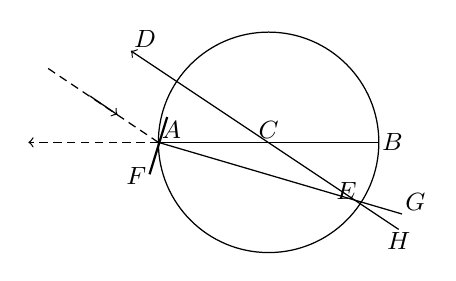
\begin{tikzpicture}[x=14mm,y=14mm,line width=.45pt,every node/.style={font=\small,inner sep=1pt}]
\draw (0,0) circle (1);
\draw (-1,0)--(1,0);
\draw[<-] (-1.25,.83)--(1.18,-.79);
\draw (-1,0)--(1.21,-.65);
\draw[line width=.8pt] (-1.08,-.29)--(-.92,.23);
\draw[densely dashed,->] (-1,0)--(-2.18,0);
\draw[densely dashed] (-2,.67)--(-1,0);
\draw[->] (-1.62,.42)--(-1.37,.25);
\node[above right] at (-1.25,.83) {$D$};
\node[above right] at (-1,0) {$A$};
\node[above] at (0,0) {$C$}; \node[right] at (1,0) {$B$};
\node[above left] at (.83,-.55) {$E$};
\node[below left] at (-1.08,-.20) {$F$};
\node[above right] at (1.21,-.65) {$G$};
\node[below] at (1.18,-.79) {$H$};
\end{tikzpicture}
\end{center}
\vfill\noindent\hfill61*

\clearpage
\noindent\makebox[0pt][l]{\fontsize{13}{16}\selectfont 484}\hfill{\small\textbf{BEMERKUNGEN.\quad HELIOTROP.}}\hfill\null\par\medskip
\begingroup\small
\noindent wird mithin, wenn das Fernrohr $HD$ auf die Sonne gerichtet ist, der Spiegel $F$ das Licht in der Richtung
$CA$ reflectiren. Um den Gegenstand, dem Licht zugesandt werden soll, in diese Richtung zu bringen, wird
das Instrument, dessen Horizontalaxe $AB$ von einer sich auf einem Dreifuss erhebenden Säule getragen
wird, so aufgestellt, dass das Object im Fernrohr $HD$ erscheint, wenn dieses der Axe $BA$ parallel ist.
Damit der Spiegel diese Beobachtung nicht hinderte, war er an einem Ringe befestigt.

Im Jahre 1821 hatte \textsc{Gauss} nur einen Heliotrop (vergl. S.~349 und 390), 1822 und 1823 je 3 (vergl.
S.~355 und 470), 1824 und 1825 (nach den Arbeitsberichten) je 4 Heliotrope im Gebrauch. Zu ihrer Bedienung
standen ihm neben den drei ständigen Gehülfen bei der Gradmessung (\textsc{Müller}, \textsc{Hartmann} und
\textsc{J.~Gauss}) 1824 noch zwei andere (Studiosus \textsc{Klüver}, der von der Stadt Bremen gestellt war, und Studiosus
\textsc{Baumann}), 1825 nur ein Gehülfe (\textsc{Klüver}) zur Verfügung.
\par\hfill\textsc{Krüger.}\par\endgroup
\vspace{20mm}
\begin{center}\rule{40mm}{.4pt}\end{center}

\clearpage
\vspace*{40mm}
\begin{center}{\Large\bfseries MESSUNGSFEHLER.}\end{center}
\clearpage\null\clearpage
\vspace*{14mm}
\begin{center}
{\Large\bfseries NACHLASS UND BRIEFWECHSEL.}\par\vspace{10mm}
[Über die bei der Landestriangulirung erforderlichen Instrumente.]
\end{center}
.\ .\ .\ .\ .\ .\ Bei einer ausgedehnten trigonometrischen Vermessung sind allerdings
Winkelmessungswerkzeuge von verschiedenem Range zu den einzelnen
Arbeiten anzuwenden. Der Rang bestimmt sich nach der grössern oder geringern
Schärfe, die mit jedem Instrumente zu erreichen ist, und wird nicht
sowohl durch eine grössere oder geringere Vollkommenheit in der Ausarbeitung,
als durch die Dimensionen des Werkzeuges bestimmt. Es liessen sich
darin viele Abstufungen machen; ich beschränke mich aber auf eine Rangirung
in 3 Klassen.

Die in München verfertigten Theodolithen von 12 Zoll Durchmesser können
zu den feinsten Winkelmessungen auf der Erde gebraucht werden. Zum zweiten
Rang zähle ich die Repetitionstheodolithen von 8 Zoll Durchmesser aus der
\textsc{Reichenbach-Ertel}schen Werkstatt; diese dienen für secundäre Messungen.
Zu noch mehr untergeordneten Messungen sowie für die Recognoscirungsarbeiten
sind noch kleinere Theodolithen dritten Ranges zureichend, wobei
allenfalls das Repetiren wegfallen kann.

Ein Theodolith vom ersten Range \textls[120]{könnte} allerdings für \textls[120]{alle}, auch
untergeordnete Arbeiten gebraucht werden. Der Grund, warum man das im
allgemeinen nicht thut, ist, theils die grössern Instrumente zu schonen, theils
weil jene ihrer Natur nach schwerer transportabel sind, und bei ihrer Aufstellung
viel mehr Zurüstungen erfordern.

Bei den eigentlichen Gradmessungsarbeiten, die zunächst nur einen wissenschaftlichen
Zweck hatten, habe ich nur einen Theodolithen ersten und ein
